\section{Текстээс зураг үүсгэх}
\subsection{Database дээр зурагний мэдээлэл хадгалах table нэмэх}
Database-н table дээр өөрчлөлт оруулахдаа бид sqlalchemy ашиглаж байгаа ба доор бичсэн моделийн дагуу бид migrate хийх юм. Үүний тулд back-end ажиллаж байгаа Docker container-лүү shell нээж төслийн root хэсгээс
\begin{lstlisting}[language=bash]
	alembic revision --autogenerate -m "your commit message"
\end{lstlisting}
гэсэн коммандын ашиглан өөрлөлт оруулах мэдээллиг үүсгэн. Дараа нь
\begin{lstlisting}[language=bash]
	alembic upgrade head
\end{lstlisting}
комманд хийснээр Датабазын модел бүрэн өөрчлөгдөнө.

\begin{lstlisting}[language=Python,caption={Table-рүү оруулсан өөрчлөлт},frame=single]
	class User(Base):
		# ...
		# Other table information

		text_title_string = Column(String(255), nullable=False, default="")
		text_title_color = Column(String(255), nullable=False, default="#000000")
		text_title_font_size = Column(Integer, nullable=False, default=0)
		text_title_font_name = Column(String(255), nullable=False, default="")
		text_title_is_vertical = Column(Integer, nullable=False, default=0)
	\end{lstlisting}

\subsection{API үүсгэх}
Back-end дээр API үүсгэхэд анхаарах хэдэн зүйл бий.
\begin{enumerate}
	\item Validation хийх ингэснээр хэрэглэгчээс ирсэн мэдээллийг шалгаж нэг ёсондоо ажиллахад  ямар нэгэн асуудалгүй болгож байгаа юм. Хэрэв буруу мэдээлэл хүсэлт маягаар ирвэл \textbf{
		      422 Unprocessable Entity}
	      гэсэн хариу буцаана.

	\item Dependency injection байдлаар user-н token-г шалгана ингэснээр хэрэглэгчийн нэвтрэлтийг шалгаж байгаа юм. Хэрэв хэрэглэгч нэвтрээгүй бол \textbf{
		      401 Unauthorized}


\end{enumerate}
\begin{lstlisting}[language=Python,caption={Зураг буцаан user-лүү илгээх endpoint},frame=single]
	from fastapi import APIRouter, Depends, status
	from sqlalchemy.orm import Session
	from app import schemas
	from app.feature.pillow import pillow_text_generator, preview_text
	from app.models.user import User
	from app.v1 import deps
	router = APIRouter()
	
	@router.post("/", status_code=status.HTTP_201_CREATED)
	def pillow_text(
			*,
			obj_in: schemas.PillowBase,
			db: Session = Depends(deps.get_db),
			_: User = Depends(deps.get_current_user),
	):
			return preview_text(
					text=obj_in.text,
					is_vertical=obj_in.is_vertical,
					color=obj_in.color,
					font_size=obj_in.font_size,
					strokewidth=obj_in.stroke_width,
					bordered=obj_in.bordered,
					PPI=obj_in.PPI,
			)
	\end{lstlisting}

\subsection{Үүсгэсэн API дуудах}
Энэхүү endpoint-руу user үүсгэх зурагнийхаа текст мэдээллийг JSON хэлбэрээр POST request явуулна. Frontend-с үүсгэсэн Endpointoo ашиглахдаа responseType-г нь arraybuffer болгож байгаа юм ингэснээр base64 image interneteer явуулснаас харьцангуй бага bandwidth ашиглах юм. Үүний дараагаар авсан датагаа decode хийж base64 img болгон хэрэглэгчид харуулна.


\begin{lstlisting}[language=JavaScript,caption={Endpoint дуудах function},frame=single]
	async preview_text_to_image({ _ }, { data }) {
    const result = await this.$axios.post(`text_image/`, data, {
      responseType: 'arraybuffer',
    })
    if (result.status === 200) {
      const b64 = btoa(String.fromCharCode(...new Uint8Array(result.data)))
      const imgData = 'data:' + result.headers['content-type'] + ';base64,' + b64
      return imgData
    } else {
      console.log('error')
    }
  },
\end{lstlisting}

\section{Business logic-г хийх}
Ямар ч request client талаас ирж болох учраас үүнийг сервер дээр боловсруулахын өмнө, validation хийх нь зөв билээ. Үүний тулд Pydantic ашиглаж байгаа юм. Pydantic нь Python дээр зориулсан validation library юм. Үүнийг ашиглан бид үүсгэсэн PillowBase class-н мэдээллийг шалгаж байгаа юм. Хэрэв буруу мэдээлэл ирвэл 422 Unprocessable Entity гэсэн хариуг буцаана.
\begin{lstlisting}[language=Python,caption={Pydantic Validator},frame=single]
	from pydantic import BaseModel
	class PillowBase(BaseModel):
    text: str
    font_path: str
    is_vertical: bool = False
    font_size: Optional[int] = 90
    color: Optional[str] = "#000000"
    bordered: Optional[bool] = True
    stroke_color: Optional[str] = "#ffffff"
    stroke_width: Optional[int] = 3
    gaps: Optional[int] = 3
    PPI: Optional[int] = 300
\end{lstlisting}

Өмнөх API-г зөвхөн хэрэглэгч ямар хэлбэр дүрстэй зураг үүсгэснээ харах зорилготой байсан бол яг production орчинд хэрвээ тэрхүү үүсгэсэн зураг нь таалагдсан бол, текстээс үүсгэсэн зураг материалд ашиглахад тэс өөр логик ашиглах юм.

\begin{figure}
	\centering
	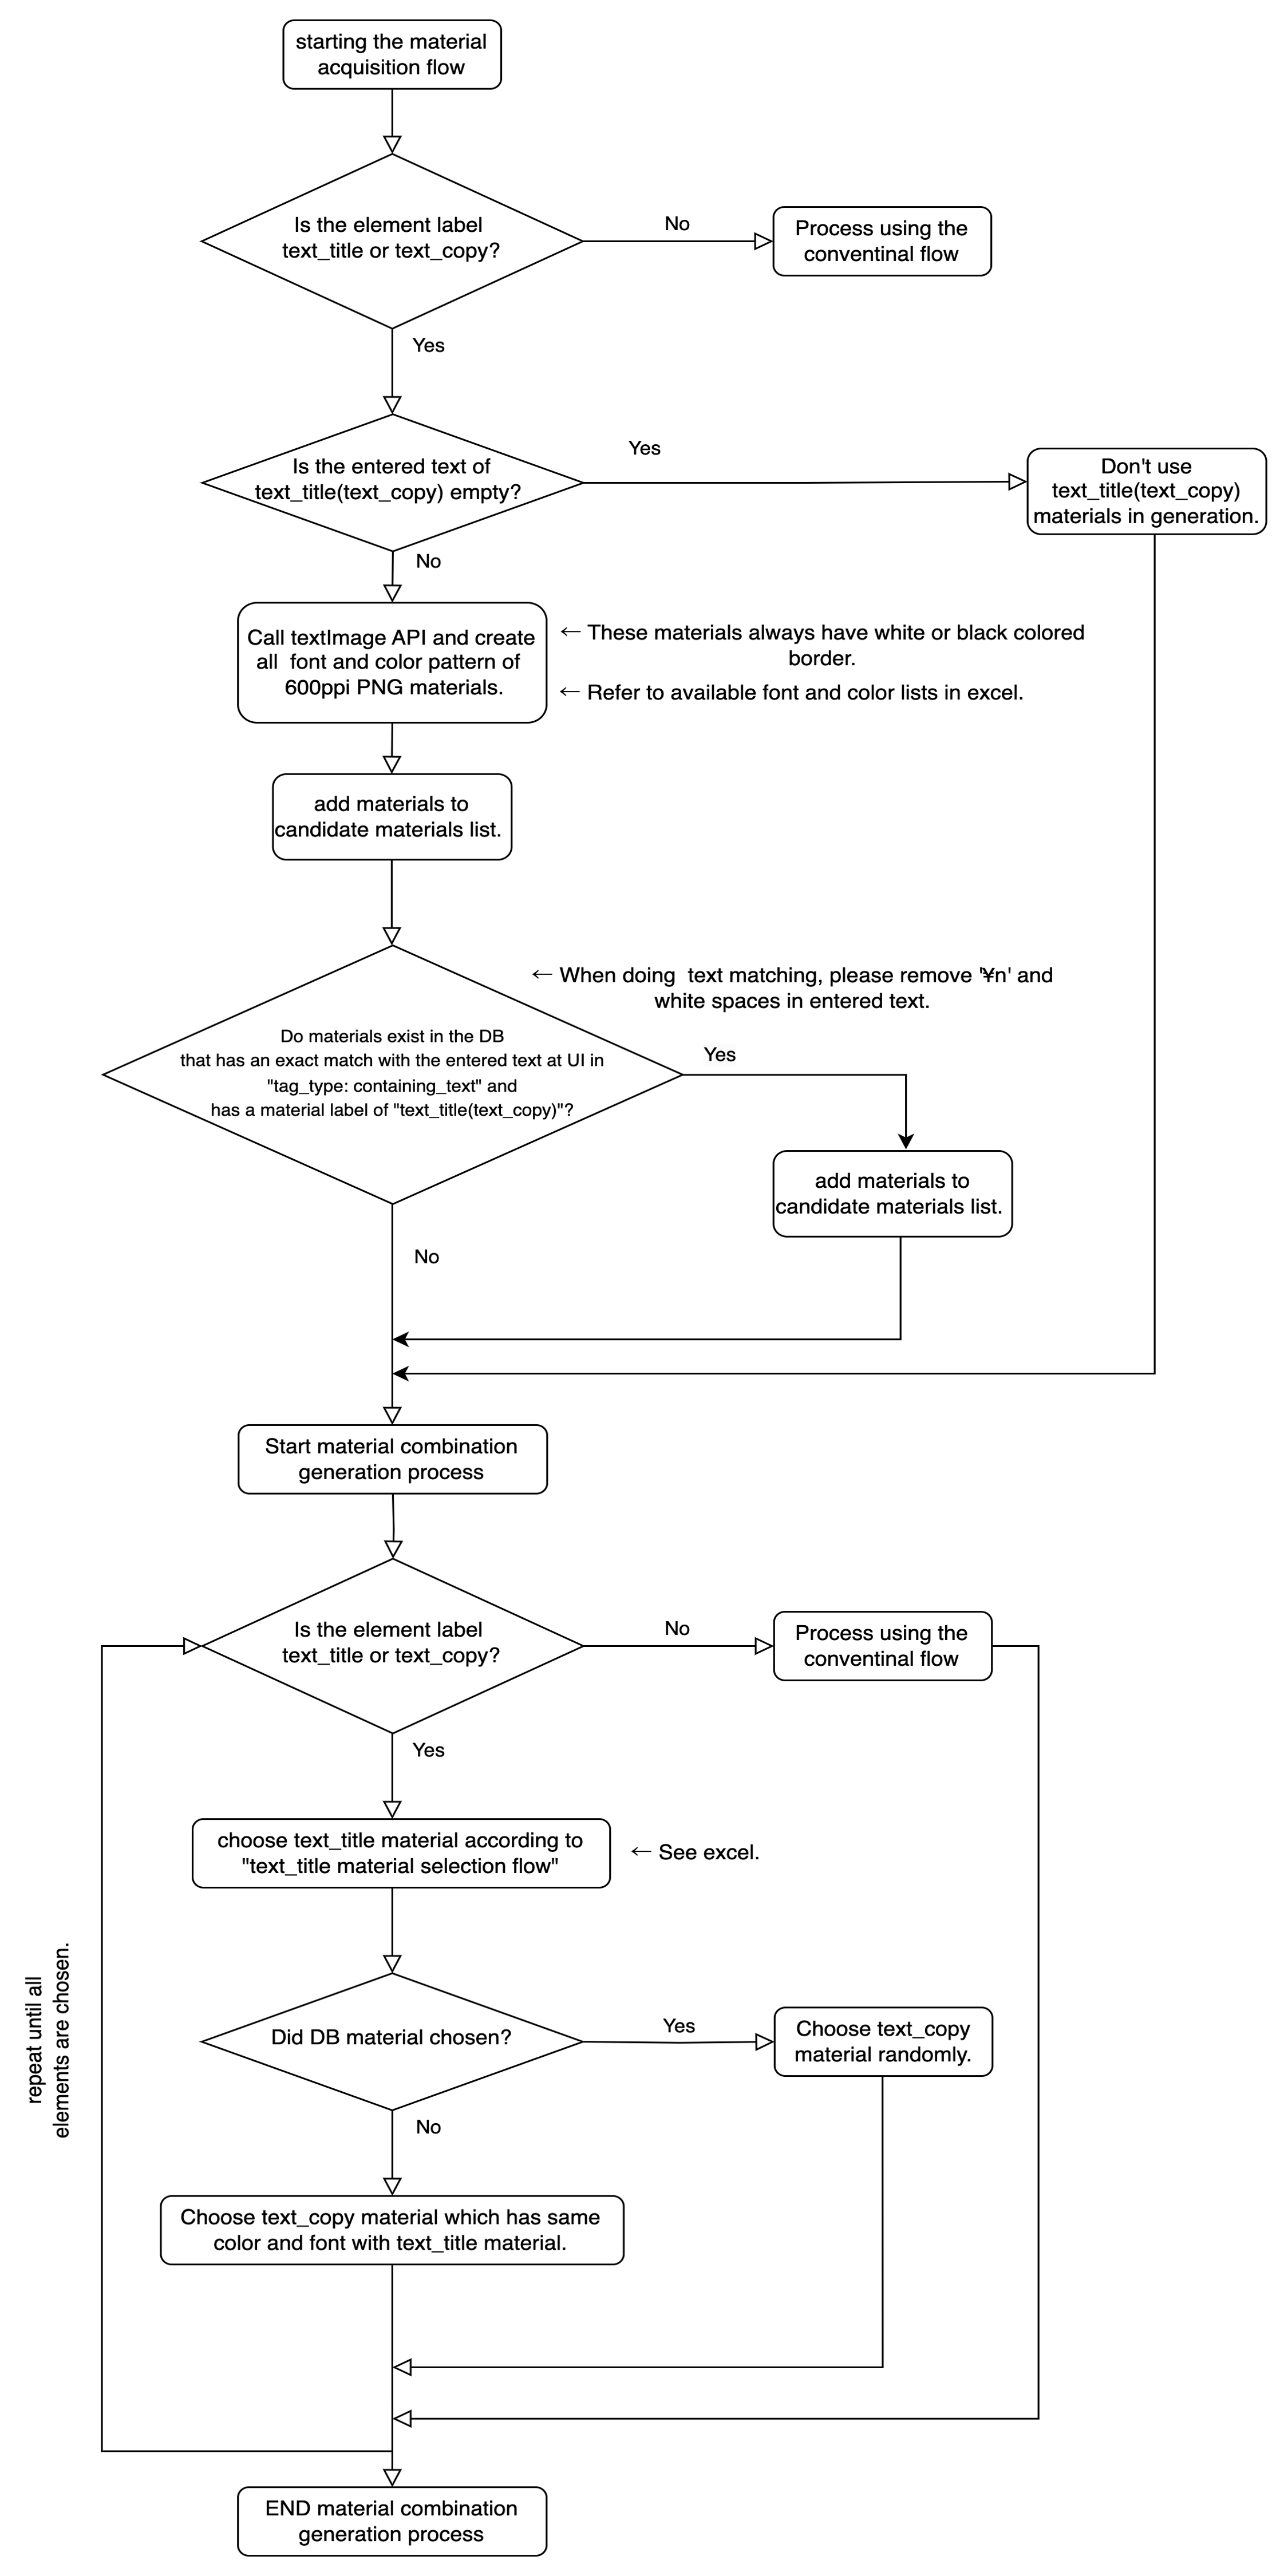
\includegraphics[scale=0.6]{src/pictures/algorithm1.png}
	\caption{Алгоритм}
\end{figure}
\subsection{Алгоритмын тайлбар}
Дээрх зурганд харуулсан Алгоритмыг ерөнхийд нь тайлбарлавал, хэрэглэгчийн зураг үүсгэхийг хүссэн тексттэй адилхан агуулгатай өгөгдөл database дээр байгаа эсэхийг шалгах юм. Хэрэв тийм өгөгдөл олдвол тухайн өгөгдлийн цаашид үүсгэх шошгонууд дээрээ жин өгч магадлал тооцон ашиглах юм.
Ингэхдээ текстээс зураг үүсгэдэг алгоритмыг ашиглан 8 өнгө 3 фонт дээр төрөл бүрийн зурагнууд үүсгэж түүнийгээ database дээр олдсон зурагнуудтай нийлүүлэн магадлал тооцно.
\begin{figure}
	\centering
	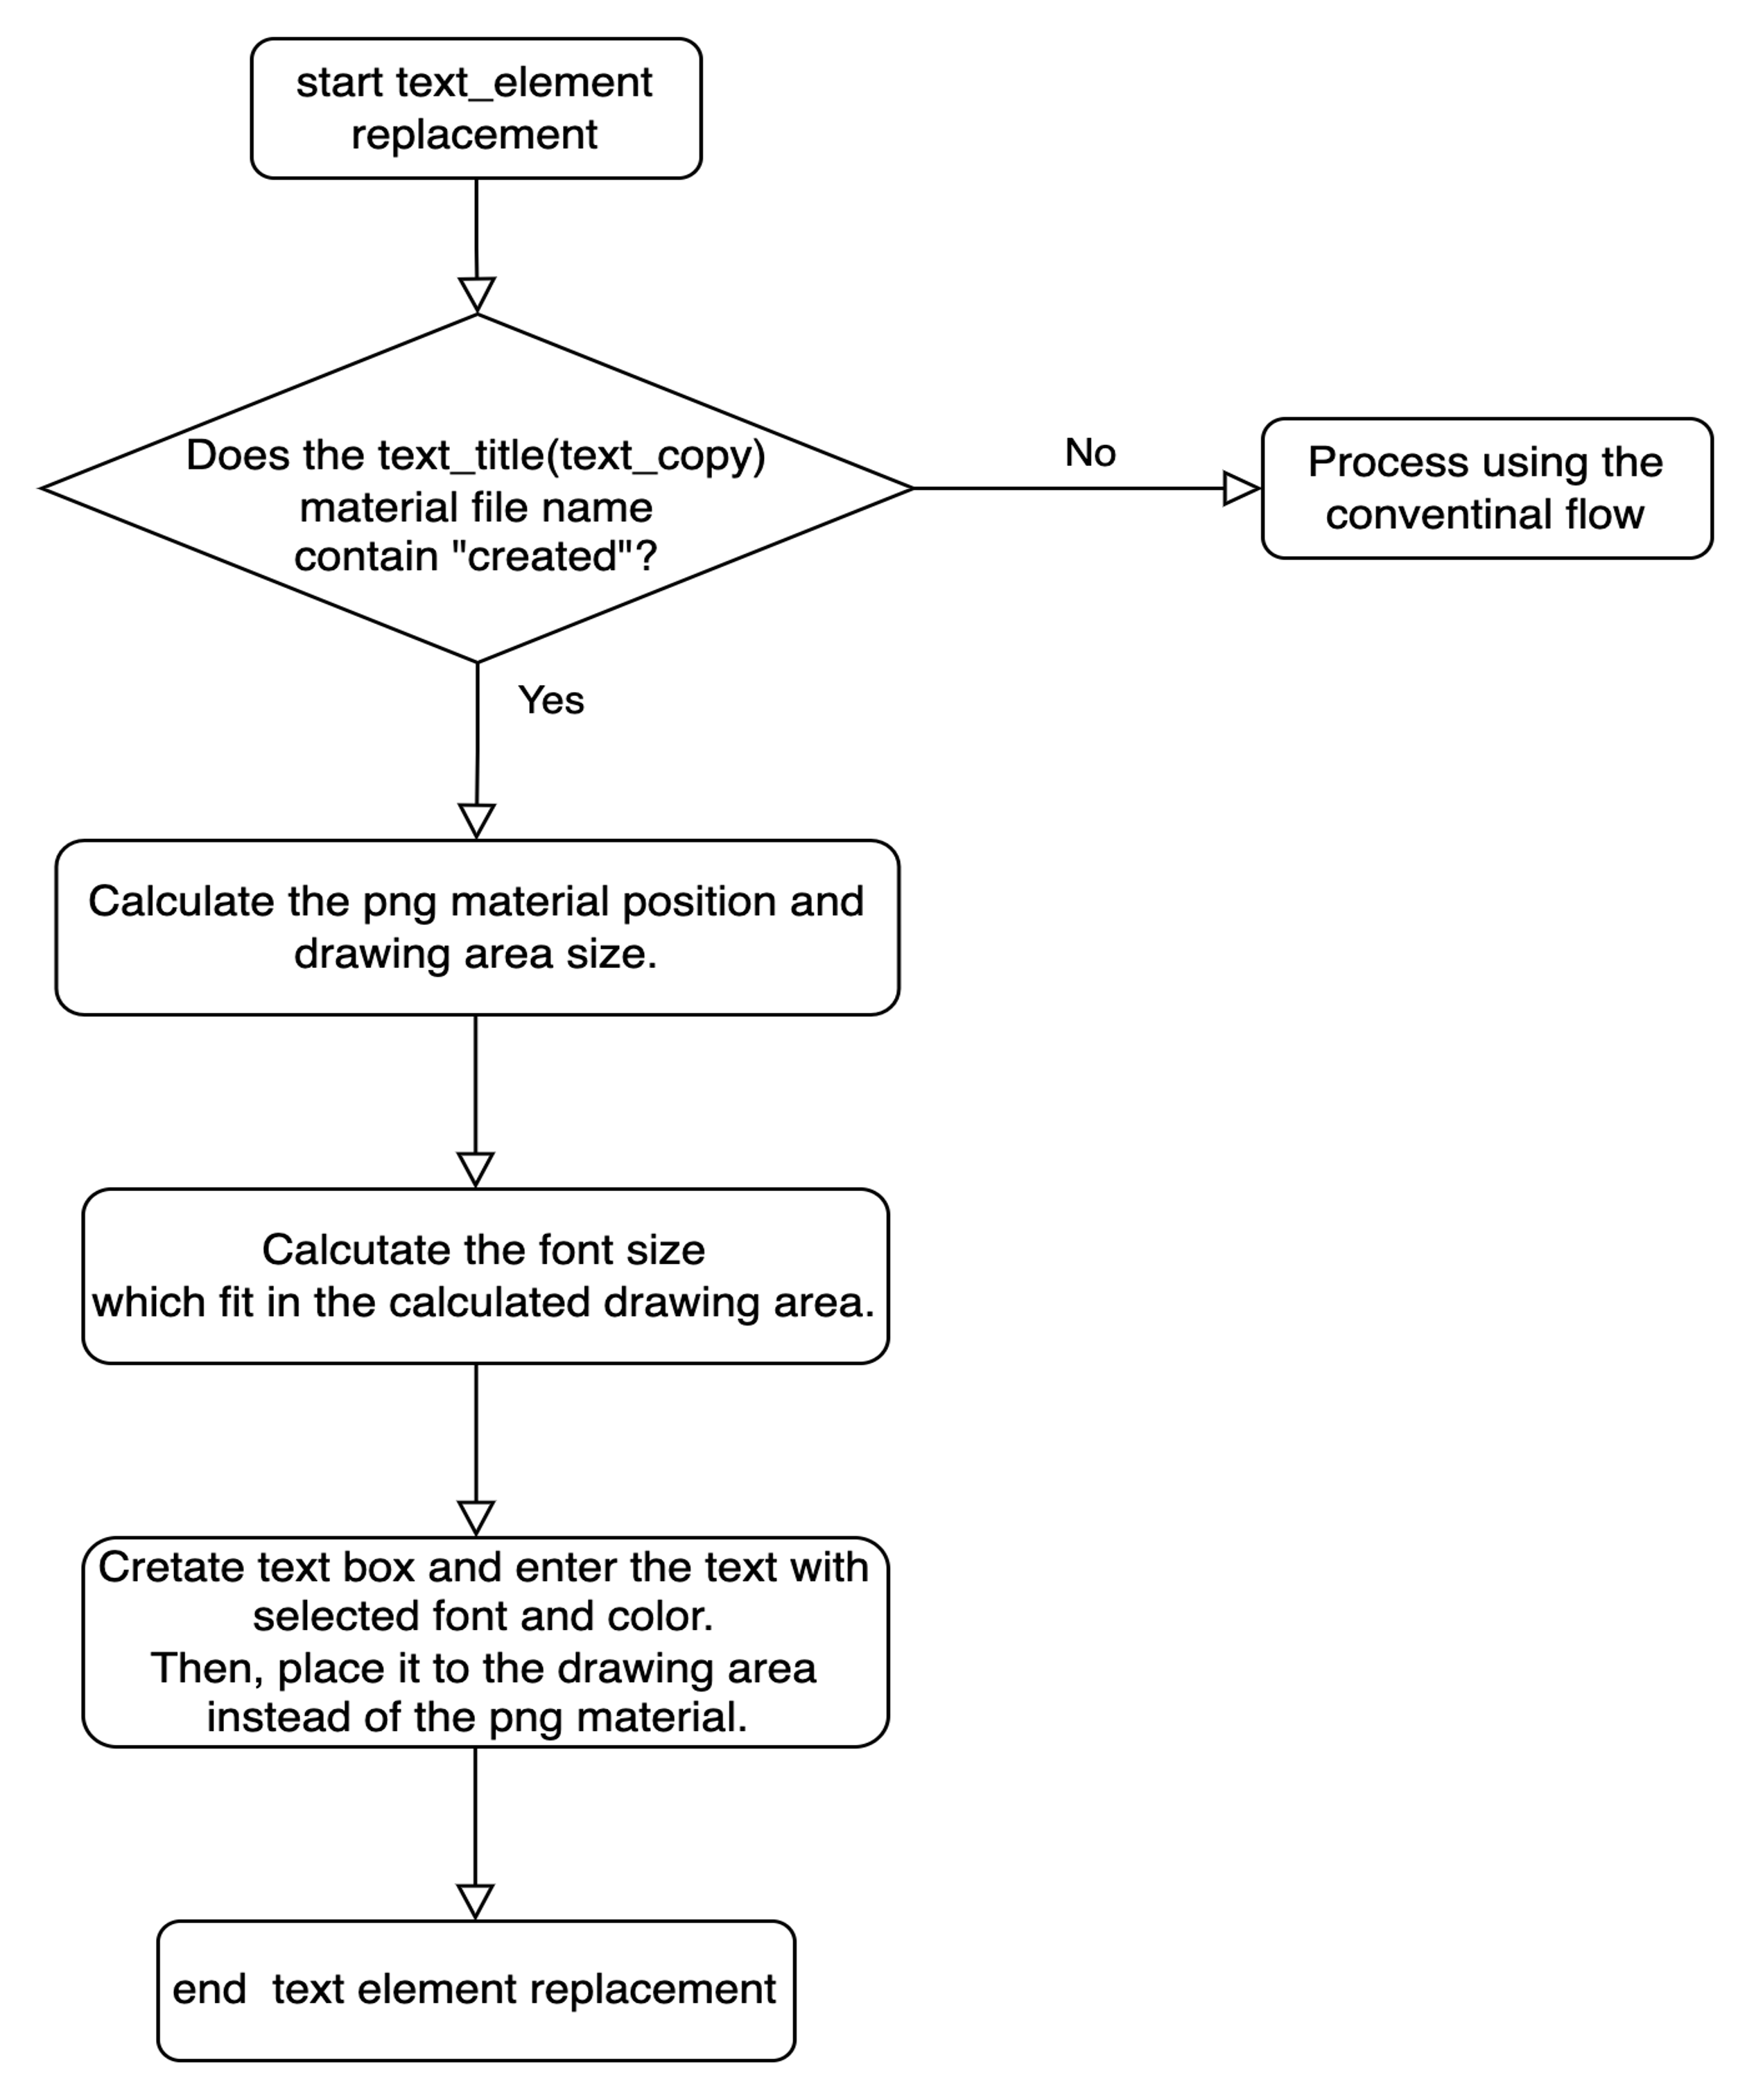
\includegraphics[scale=0.6]{src/pictures/algorithm2.png}
	\caption{Алгоритм-2}
\end{figure}

\begin{lstlisting}[language=Python,caption={Сонголт хийх код},frame=single]
	if registered_materials_from_db:
	item_list.extend([black, other, db_item])
	item_weight.extend([0.7 * 1 / 3, 0.3 * 1 / 3, 1 / 3])
else:
	item_list.extend([black, other])
	item_weight.extend([0.7, 0.3])
\end{lstlisting}

\subsection{Ажиллах дараалал}
\begin{enumerate}
	\item Хэрэглэгчийн оруулсан текстээс \verb|\n| ялгаж хэдэн мөр байхыг гаргана.
	\item Хэрэглэгчийн оруулсан фонт мөрийн тоо, нэг мөр дэх үсгийн тооноос хамаарч өөр өөр байх хоосон зургуудийг үүсгэнэ.
	\item Хоосон зургуудруугаа текстийг нэг нэгээр нь нэмнэ.
	\end{enumerate}